

bllblnlb
\subsection{Risk Analysis Methodology}
The methodology adopted to conduct the risk analysis is described as following steps: \\Step 1: Identify potential risks \\Step 2: Determine probability \\Step 3: Determine Impact\\  As long as all possible risks are identified after brainstorming, they will be assessed according to the probability and impact respectively. Each aspect has a scale of 1, 3, and 9. A bigger number implies that the risk is more likely to happen or has a more serious consequence. Those risks of interest will be analyzed further based on their risk rating, which is defined as the product of probability and impact. 
\begin{figure}[h!]
\centering
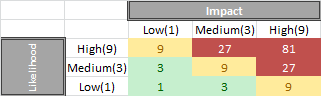
\includegraphics[scale=1.0]{Pictures/riskmatrix.png}
\caption{Risk Matrix}
\label{fig:riskmatrix}
\end{figure}

A risk matrix is shown in Table 1. The risks that lies in the upper right in red exceeds the level of tolerance and needs to be made action plan for. 
\subsection{Risk Log}
After the possible risks are identified, they are kept in table 2 following the priority of risk rating. The possible risks with high risk rating are marked in red and will be provided with an action plan below. 

\subsection{Action Plan}

An action plan is made for those risks with the highest likelihood and/or consequence. So the risks with risk rating above 9 are provided with the corresponding action plan.



